\documentclass[12pt]{article}
\usepackage[margin=2cm]{geometry} 
\usepackage{titling}
\usepackage{graphicx}
\usepackage{float}
\usepackage[hidelinks]{hyperref}
\usepackage[italian]{babel}

\setlength\parindent{0pt}
\setlength{\parskip}{1em}
\setlength{\droptitle}{-2cm}

\title{Istruzioni d'uso Thymio}
\author{Università della Svizzera Italiana}
\date{Versione \today}


\begin{document}
\maketitle
\tableofcontents
\newpage


\section{Installazione}

	\subsection{Windows}
	
		Recarsi all'indirizzo \url{https://www.thymio.org/program/} e scaricare il software Aseba cliccando sul bottone \texttt{Download} sotto il logo Windows.\\
		Aprire il file .exe scaricato e proseguire con l'installazione guidata. Scegliere ``ThymioII package" quando richiesto.
		
	\subsection{MacOS}
	
		Recarsi all'indirizzo \url{https://www.thymio.org/program/} e scaricare il software Aseba cliccando sul bottone \texttt{Download} sotto il logo Apple.\\	
		Aprire il file .dmg scaricato e trascinare la cartella Aseba in Applicazioni.
		
	\subsection{Linux}
	
		Recarsi all'indirizzo \url{http://wiki.thymio.org/en:linuxinstall} e seguire le istruzioni per la piattaforma in uso.
			

\section{Collegamento del robot}

	Prima di utilizzare qualsiasi software, è necessario collegare almeno un robot al computer (vedi sezione \ref{network} per multipli robot). Questo può essere fatto in due modi: tramite cavo o wireless (se supportato).
	
	\subsection{Cavo USB}
	
		Collegare il cavo in dotazione ad una porta libera sulla propria macchina e alla porta microUSB sul retro del Thymio. Il robot si accenderà automaticamente non appena rilevata la connessione.
		
	\subsection{Dongle wireless (se disponibile)}
	
		Collegare il dongle ad una porta libera sulla propria macchina e accendere il robot tenendo premuto il tasto centrale per circa 3 secondi.
	

\section{Software}

	\begin{figure}[h]
		\begin{minipage}{0.49\textwidth}
        			\centering
			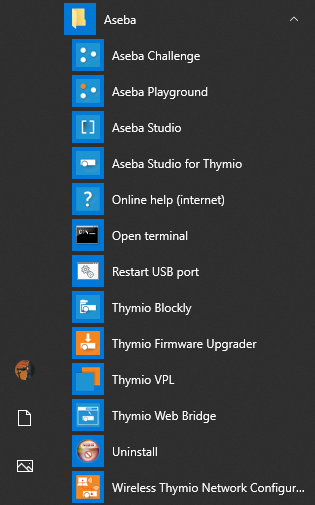
\includegraphics[width=\textwidth]{img/appsWin.png}
		\end{minipage}\hfill	
		\begin{minipage}{0.49\textwidth}
			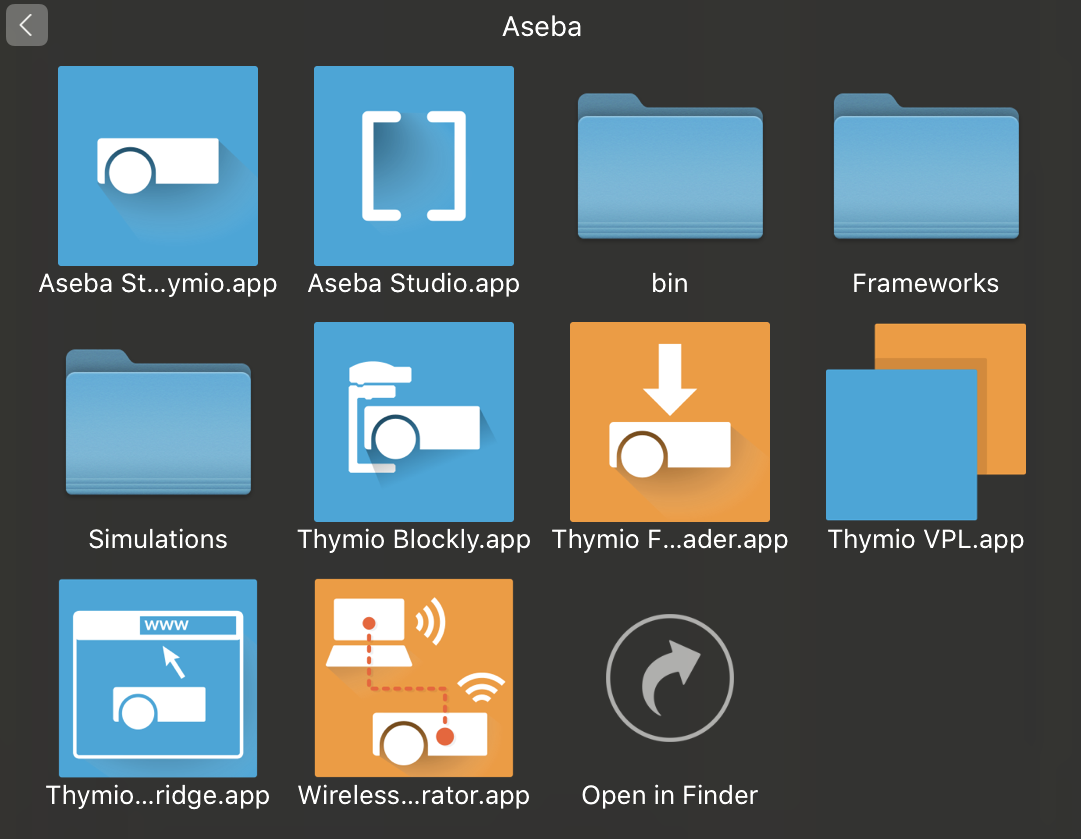
\includegraphics[width=\textwidth]{img/appsMac.png}
		\end{minipage}
		\caption{Il software a disposizione su Windows (sinistra) e Mac (destra)}
		\label{apps}
	\end{figure}
		
	\subsection{Aseba Studio}
	
		Aseba Studio è un software per programmare direttamente i robot Thymio, pensato per utenti più esperti. Per utilizzarlo è sufficiente lanciare Aseba Studio for Thymio.
		
		\begin{figure}[H]
			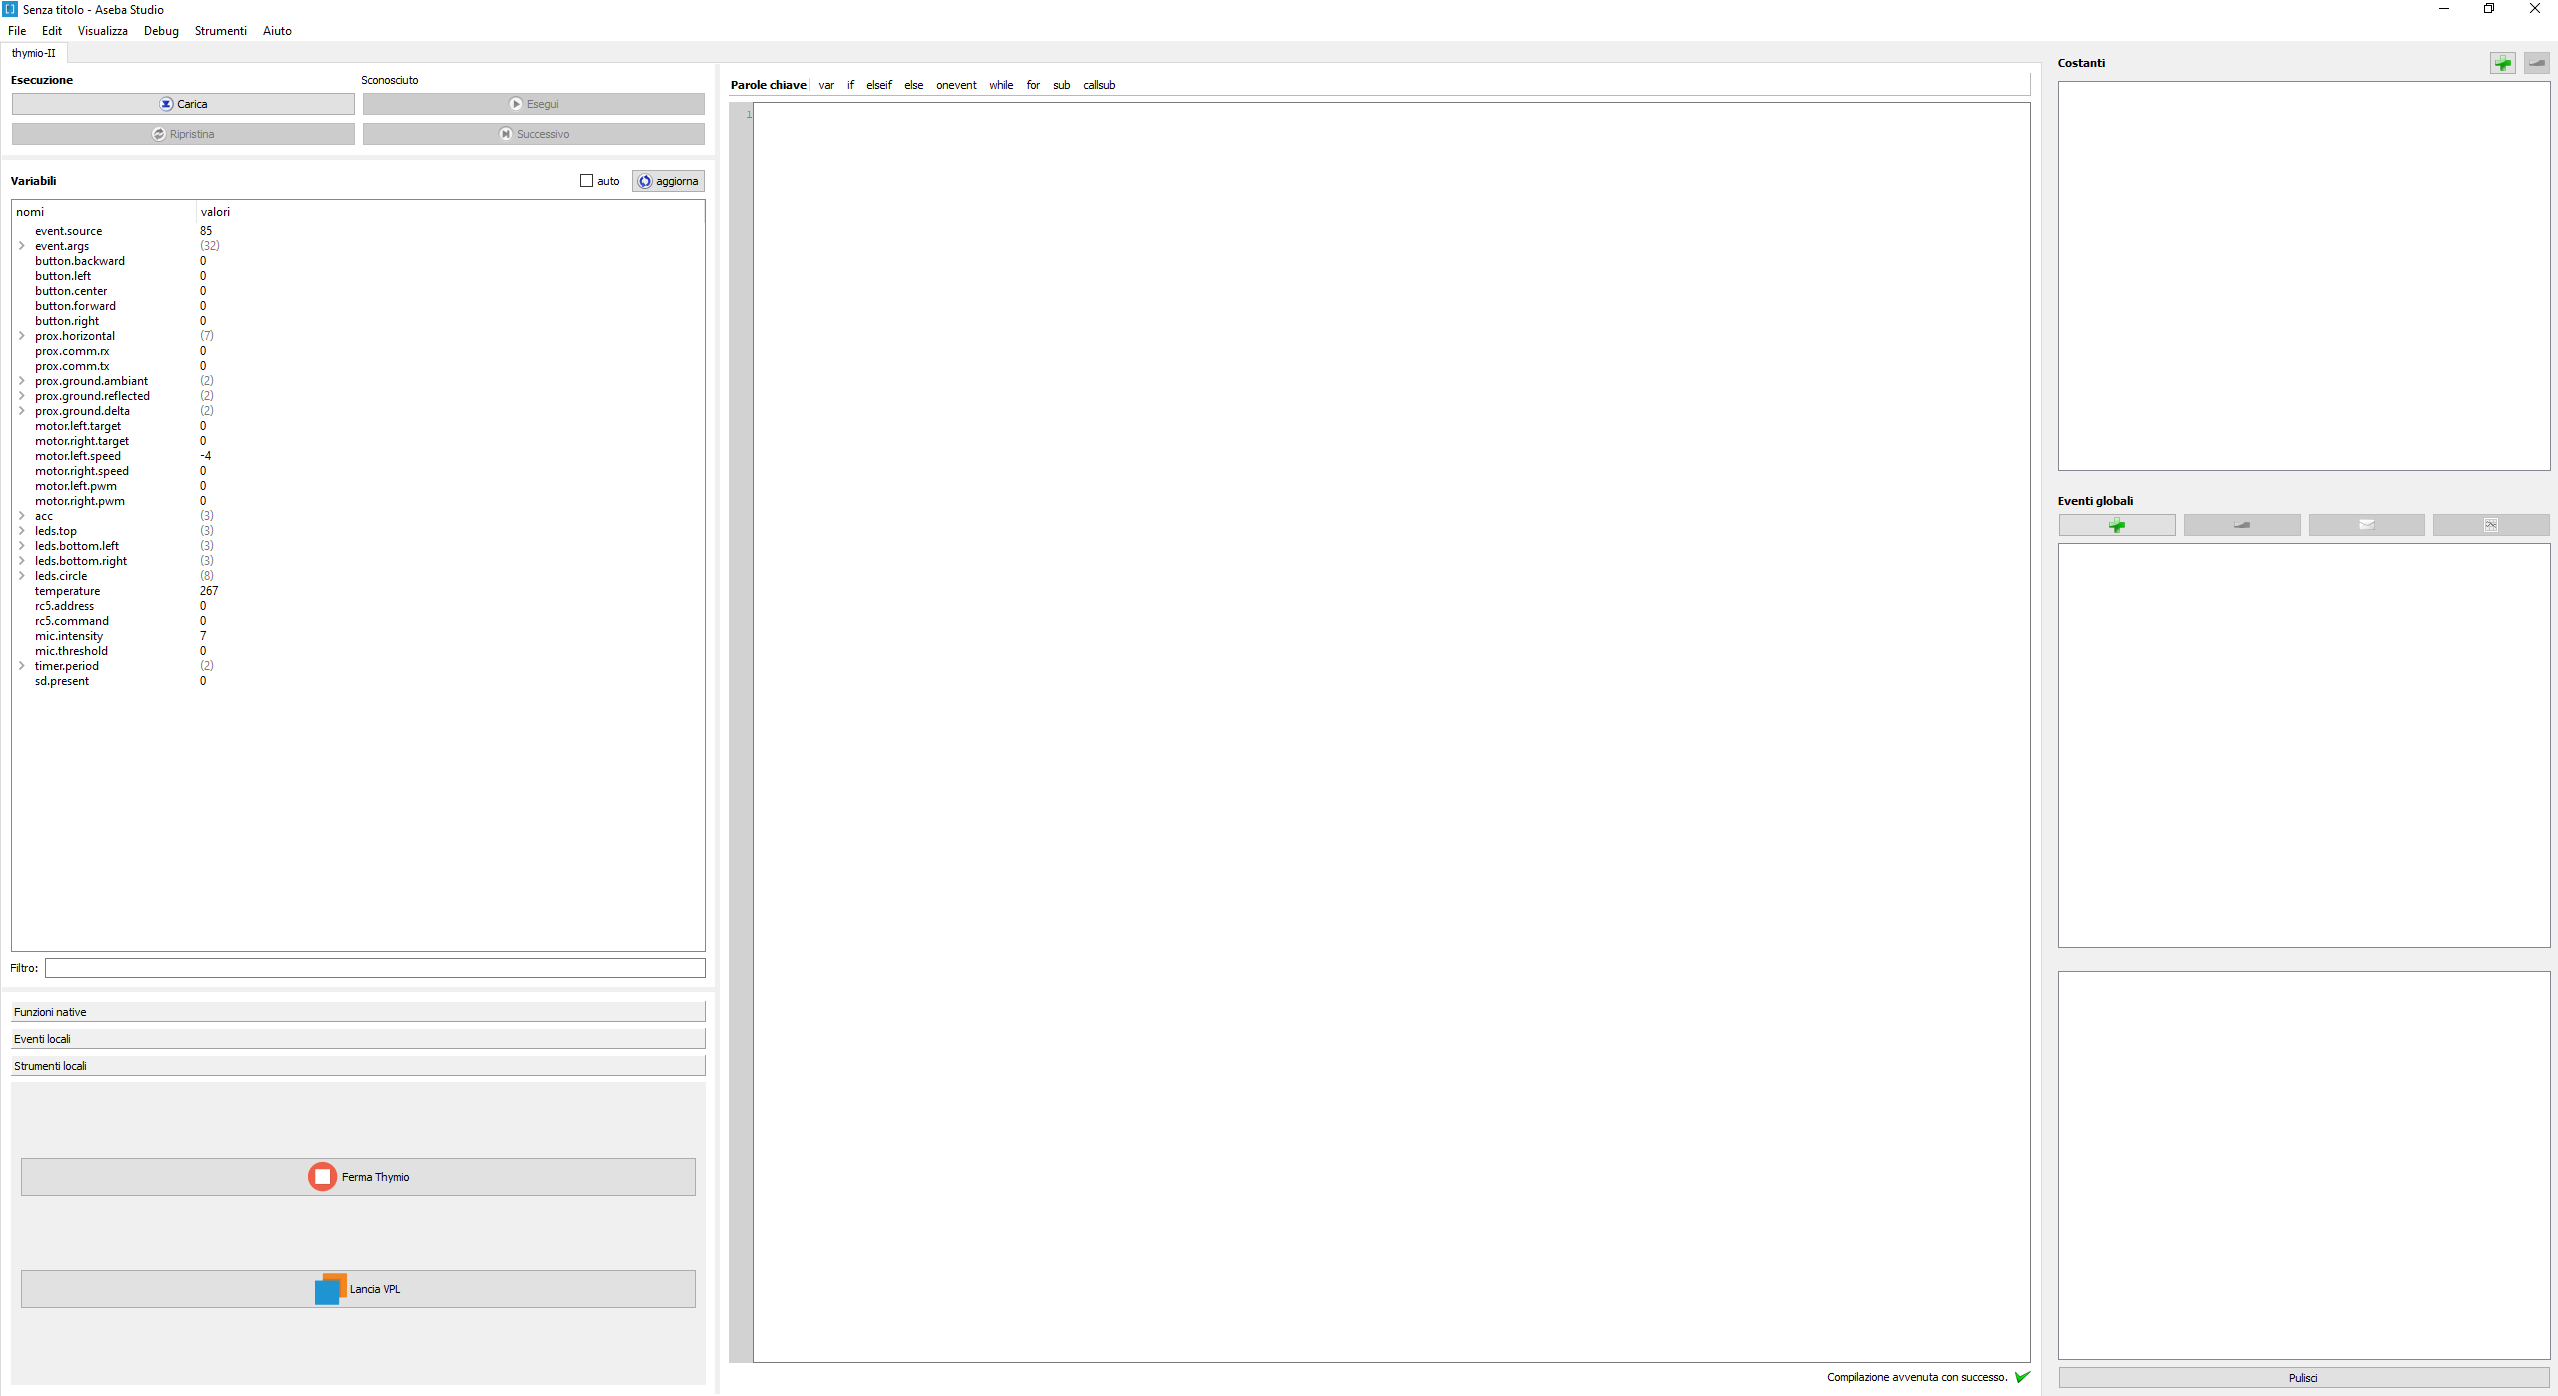
\includegraphics[width=\textwidth]{img/asebaConnIta.png}
			\caption{La finestra principale di Aseba Studio}
			\label{aseba1}
		\end{figure}		

	\subsection{Blockly}

		Blockly è un software per programmare in maniera intuitiva. Per utilizzarlo è necessario lanciare Thymio Web Bridge e in seguito Thymio Blockly.
		
		Nota: Se si riceve l'errore \textit{Unhandled Dashel exception: Connection failed (48): Cannot bind socket to port, probably the port is already in use} controllare che la porta 3000 non sia già in uso.
	
		Nota: su MacOS i due programmi verranno bloccati dal sistema siccome provengono da una fonte esterna (vedi figura \ref{macErr}). Cliccare su Annulla, in seguito recarsi in Impostazioni di Sistema, sotto Sicurezza e Privacy e cliccare su Apri Comunque. Ora è possibile avviare il software, cliccando un'ultima volta su Apri quando richiesto.
		
		\begin{figure}[H]
			\begin{minipage}{0.39\textwidth}
        				\centering
				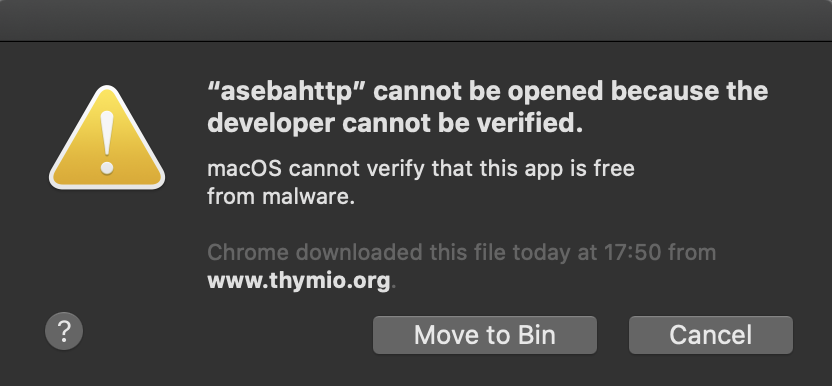
\includegraphics[width=\textwidth]{img/macWarn1.png}
			\end{minipage}\hfill	
			\begin{minipage}{0.6\textwidth}
				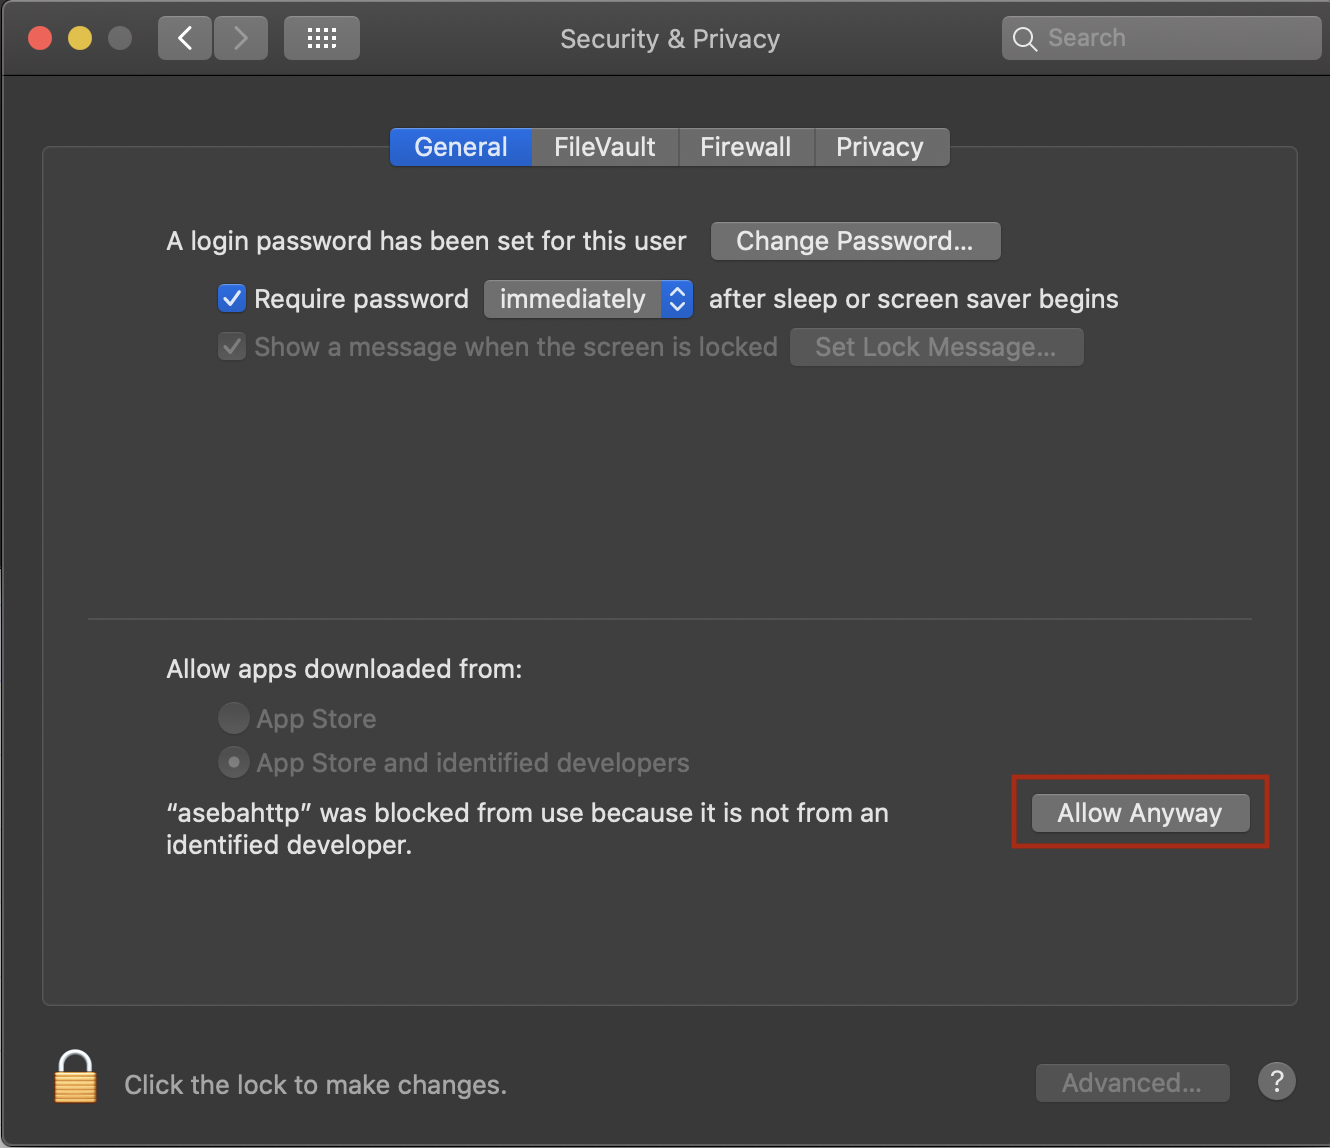
\includegraphics[width=\textwidth]{img/macWarn2.png}
			\end{minipage}
			\caption{Il messaggio di avviso di MacOS e le Impostazioni di Sistema}
			\label{macErr}
		\end{figure}
		
	\subsection{VPL}
	
		VPL (Visual Programming Language) è un software semplificato pensato per i più giovani. Per utilizzarlo è sufficiente lanciare Thymio VPL.
		
		
\section{Esempi di codice}

	\subsection{USI Showroom}
		
		Al seguente indirizzo sono disponibili diversi file con esempi di semplici programmi appositamente prodotti dall'USI:
		
		\url{https://github.com/USI-Showroom/thymio}
		
	
	\subsection{Risorse ufficiali}
	
		Ai seguenti indirizzi sono disponibili diversi tutorial ed esempi ufficiali di codice:
	
		\url{http://wiki.thymio.org/en:creations}
		
		\url{https://github.com/Mobsya/thymio-programming-exercises}
		
		\url{https://github.com/Mobsya/thymio-vpl-tutorial}
	
	
\section{Comunicazione fra robot}\label{network}

	È possibile far comunicare due robot tramite infrarossi (IR). Siccome la comunicazione avviene tramite i sensori orizzontali (cinque anteriori e due posteriori), i robot devono essere in grado di ``vedersi''.
	
	Prima di tutto è necessario attivare la comunicazione IR su entrambi i robot, dopodiché si possono usare i blocchi o i comandi specialmente previsti (rispettivamente su Blockly e Aseba studio) per trasmettere e ricevere i segnali; purtroppo al momento questa funzione non è disponibile in VPL. 
	
	Di seguito un semplice esempio dove il primo robot trasmette un segnale IR e il secondo reagisce cambiando il colore del LED superiore: 
	
	\begin{figure}[H]
		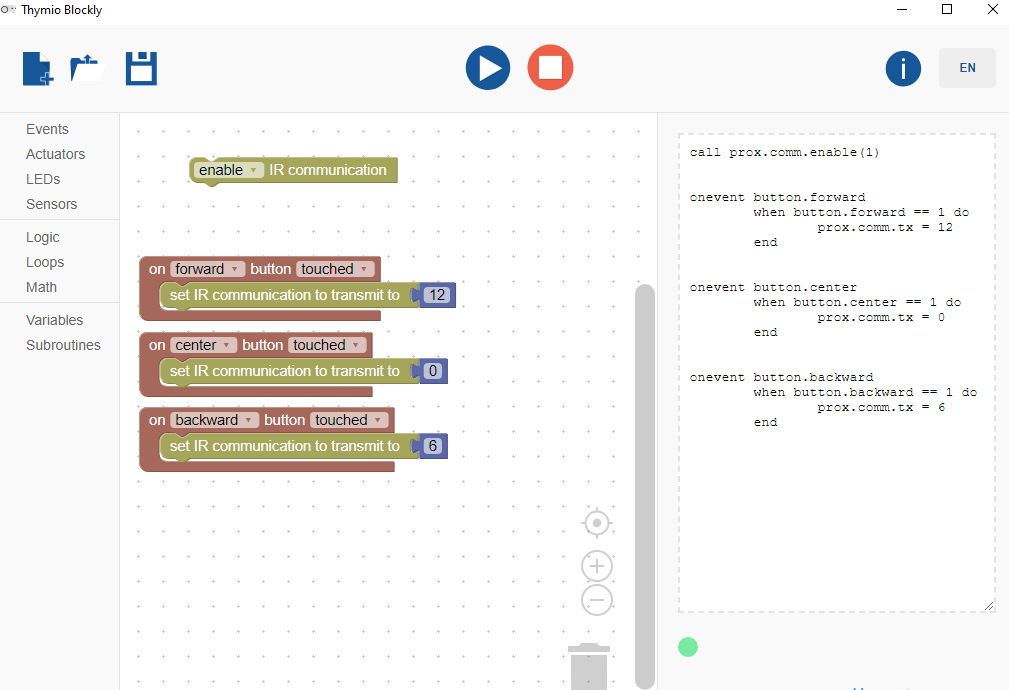
\includegraphics[width=\textwidth]{img/blocklyIR1.png}
		\label{blocklyIR1}
	\end{figure}
		
	\begin{figure}[H]
		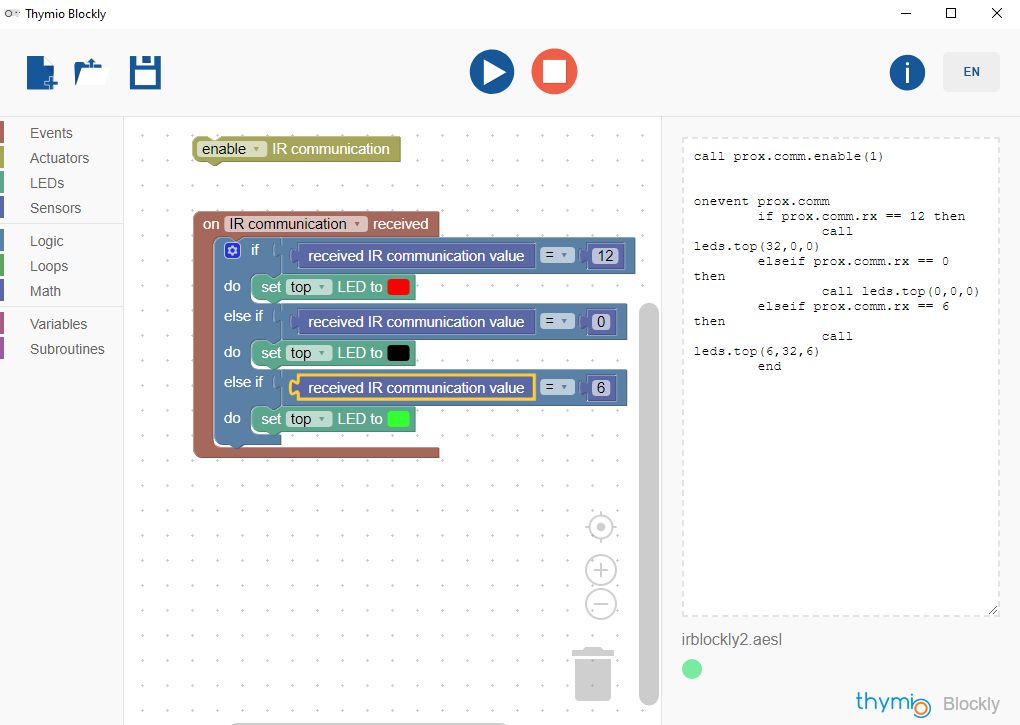
\includegraphics[width=\textwidth]{img/blocklyIR2.png}
		\caption{Un semplice esempio di comunicazione fra due robot}
		\label{blocklyIR2}
	\end{figure}
	
		
\section{Aggiornamento del firmware}

	Recarsi all'indirizzo \url{https://github.com/Mobsya/aseba-target-thymio2/releases} e scaricare il file \texttt{.hex} per la versione più recente. Collegare il robot con il cavo USB e avviare Thymio Firmware Upgrader; scegliere Custom Firmware, selezionare il file appena scaricato e cliccare su Upgrade. 
	
	\textbf{NON} scollegare o spegnere il robot durante la procedura!
	
\end{document}